\chapter{Methodology}

\section{Introduction}
The focus of this project is to explore the uses of Naive Bayes in chess and whether it is a viable alternative to current techniques. This chapter will describe the methodology that was used to implement the Naive Bayes classifier in the chess engine. For this project, the python-chess library was highly relied upon. Many different Python scripts were used during the project. The main scripts included were \texttt{data\_prep.py} where the data was preprocessed, \texttt{training.py} where the model was trained and evaluated, \texttt{features.py} where the features were calculated, \texttt{game.py} where the game was played and the most important ones \texttt{minimax\_NB\_XXX.py} where the Naive Bayes Classifier was applied to the minimax algorithm.

% \section{Random Chess Engine}

\section{Integration of Naive Bayes with Minimax}

\subsection{Data Preparation}

The dataset used for this project was obtained from Kaggle \cite{ChessGameDataset} \url{https://www.kaggle.com/datasets/arevel/chess-games}. The dataset contained over 6.2 million chess games that were played on lichess.com in July 2016. The dataset was in CSV format, making it easy to extract information and analyse. The dataset contained many features, however, the only features relevant to this project were the result of the game and the sequence of moves in Algebraic Notation form.

This project wants to explore how the classification of chess positions into wins and losses can be used to improve the minimax algorithm. For this reason, all games which resulted in a draw were not considered as well as games where one of the players resigned. The data was split into 3 different groups to explore how player expertise affects the model's learning and generalisation ability. The first group, named \texttt{master}, was all games where one of the players had an Elo rating of 2200 and above as defined by the Federation International des Echecs (FIDE). The second group, named \texttt{beginner}, were games where both players had an Elo lower than 2200. The last group, named \texttt{random} were games where players with any Elo were considered. The dataset only had 300,000 instances of master games, therefore only 300,000 instances of beginner and random games were used. This is to ensure that the experiments are fair when comparing the effect of the different datasets on the model's performance. 

The moves in Algebraic Notation would not provide the Naive Bayes classifier with enough information to classify as it would not provide context of the board state. For this reason, the python-chess library was used to simulate the games. The moves would be extracted from the CSV file, then each move would be played on the board. The CSV file would be read by using the pandas library and every 6 moves, the features of the board would be extracted and stored, this was to reduce the amount of data to train on as consecutive moves are highly correlated so would not provide more insight for the model. However, end game moves have a bigger effect on the result of the game so in this phase, every other move was used. The last move was also included since this is the move and game state that determined the result of the game. This was also when the results of the games were converted from \texttt{1-0} or \texttt{0-1} to a binary classification where 1 represented a win and 0 represented a loss. This was done to make the model easier to train and evaluate.

\subsection{Feature Selection}

Feature selection is a crucial part of how well the Naive Bayes will perform and generalise. Limited use of features can lead to underfitting and too many features can lead to overfitting. This project also wants to explore the impact different features can have on the model's performance. There were 4 feature sets used in this project. 

The first feature set, considered 4 features: material balance, piece mobility, king attack balance and positional value. Material balance is a very simple feature that considers the difference in number of pieces between the two players, where a positive value indicates a piece advantage for white and a negative value indicates a piece advantage for black. However, each piece is not of equal value in the game, for example, a queen has much more power than 2 pawns have. For this reason, the values in Table~\ref{tab:piece_values} were used \cite{shannonXXIIProgrammingComputer1950} \cite{drosteLearningPieceValues}. 


\begin{table}[h]
    \centering
    \begin{tabular}{|c|c|}
        \hline
        \textbf{Piece} & \textbf{Value} \\
        \hline
        Pawn & 100 \\
        Knight & 300 \\
        Bishop & 300 \\
        Rook & 500 \\
        Queen & 900 \\
        King & 0 \\
        \hline
    \end{tabular}
    \caption{Values of Chess Pieces}
    \label{tab:piece_values}
\end{table}

Piece mobility is the difference in the number of legal moves between the two players. The more moves available to a player suggests that they have more control over the board which could give them a tactical advantage. King attack balance is the difference in the number of pieces attacking the king. Most of these features are simple and don't consider the game state as a whole, like the position of pieces on the board. Positional value was a feature used where the location of a particular piece on the board can affect how effective it is. An example of a positional value table for a knight is shown in Table~\ref{tab:knight_positional_values}.

\begin{table}[h]
    \centering
    \begin{tabular}{|c|c|c|c|c|c|c|c|c|}
        \hline
        \textbf{} & \textbf{A} & \textbf{B} & \textbf{C} & \textbf{D} & \textbf{E} & \textbf{F} & \textbf{G} & \textbf{H} \\
        \hline
        \textbf{8} & -50 & -40 & -30 & -30 & -30 & -30 & -40 & -50 \\
        \textbf{7} & -40 & -20 & 0 & 5 & 5 & 0 & -20 & -40 \\
        \textbf{6} & -30 & 0 & 10 & 15 & 15 & 10 & 0 & -30 \\
        \textbf{5} & -30 & 5 & 15 & 20 & 20 & 15 & 5 & -30 \\
        \textbf{4} & -30 & 0 & 15 & 20 & 20 & 15 & 0 & -30 \\
        \textbf{3} & -30 & 5 & 10 & 15 & 15 & 10 & 5 & -30 \\
        \textbf{2} & -40 & -20 & 0 & 5 & 5 & 0 & -20 & -40 \\
        \textbf{1} & -50 & -40 & -30 & -30 & -30 & -30 & -40 & -50 \\
        \hline
    \end{tabular}
    \caption{Positional Value Table for Knight}
    \label{tab:knight_positional_values}
\end{table}

This table favours the knight to be in the centre of the board rather than the edge. This is because when the knight is is in the centre, it can control more squares so has more opportunity to attack and defend, whereas when it is near the edge, the knight is more restricted, especially the corners where it only has 2 possible moves.

The second feature set considered the same features as the first set but also included the control of the centre. This is defined by the number of pieces within the centre. Again, it calculates the difference between the white and black pieces in the middle. This feature was implemented as two separate features, one for the 2x2 square in the middle and one for the 4x4 square in the middle as shown in Figure~\ref{fig:centres}.

\begin{figure}[h]
    \centering
    \begin{subfigure}[t]{0.4\textwidth}
        \centering
        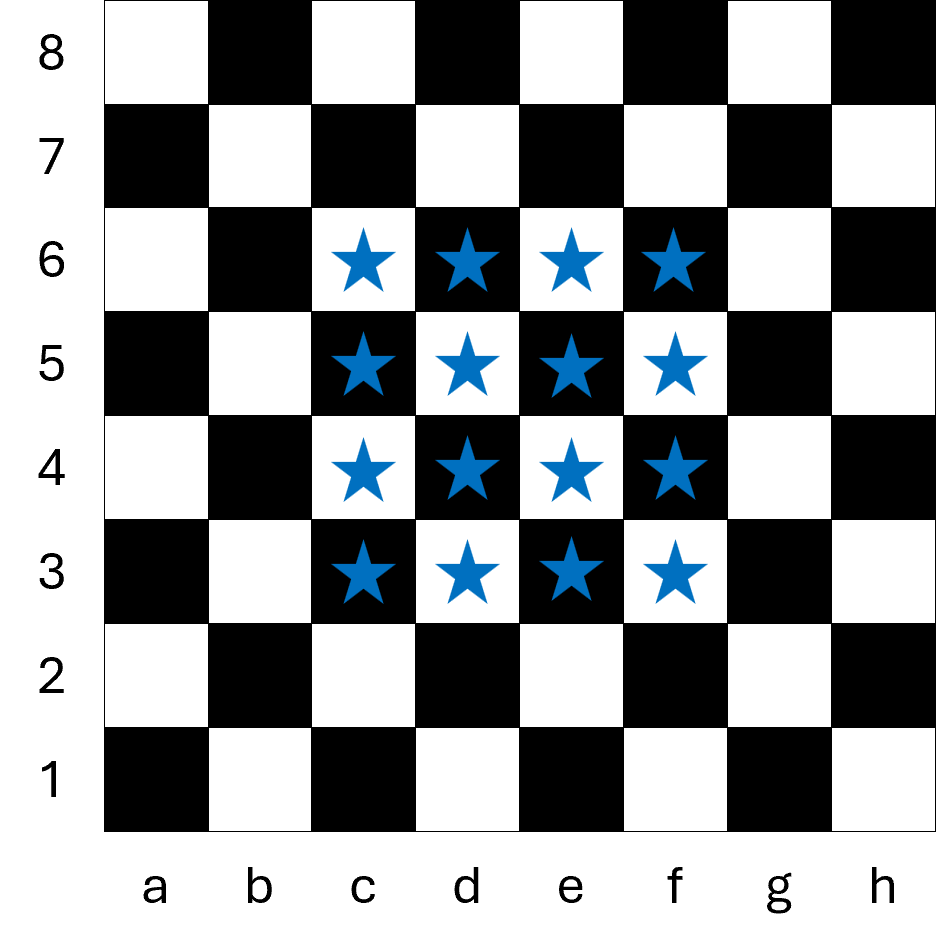
\includegraphics[width=\textwidth]{images/bigCentre.png}
        \caption{Big centre of the Board}
        \label{fig:bigcentre}
    \end{subfigure}
    \hfill
    \begin{subfigure}[t]{0.4\textwidth}
        \centering
        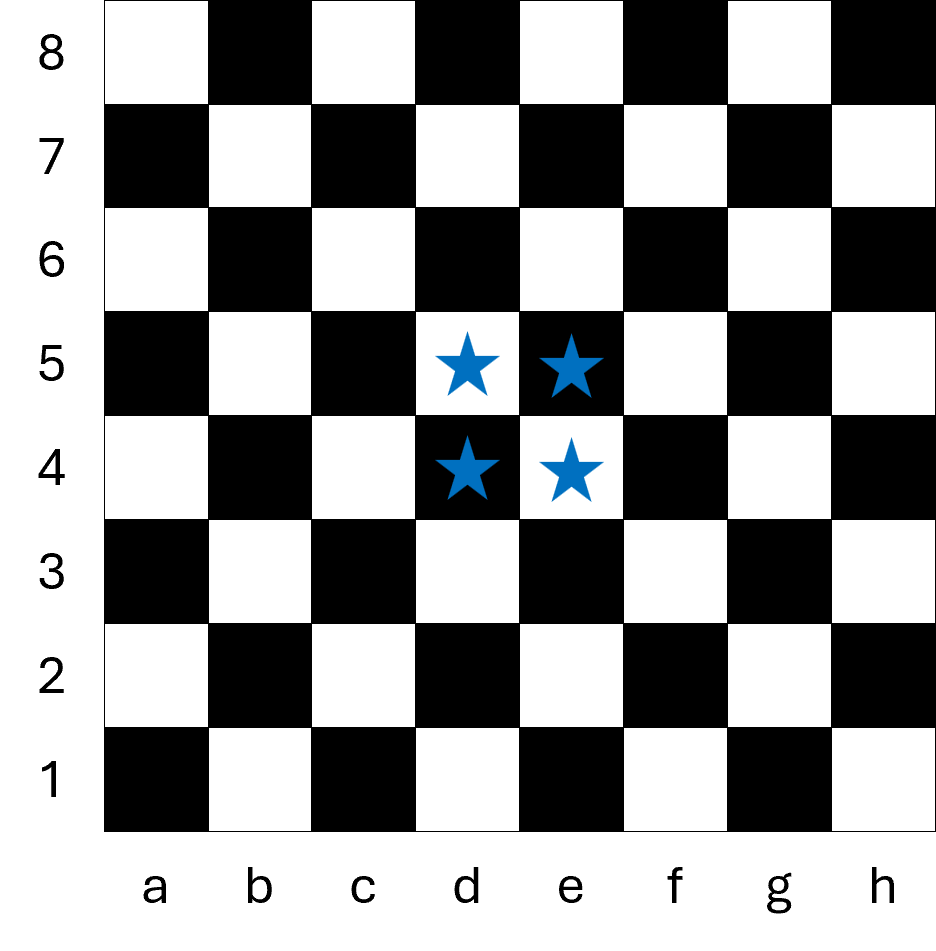
\includegraphics[width=\textwidth]{images/smallCentre.png}
        \caption{Small centre of the Board}
        \label{fig:smallcentre}
    \end{subfigure}
    \caption{Comparison of the small and big centres of the board.}
    \label{fig:centres}
\end{figure}

The third feature set explored in this research considers all of the features mentioned previously but also more complex features, specifically pawn structure. The structure of pawns can determine how much control the player has, defending its pieces and preventing advancements from the enemy. Two structures were used for this project, isolated pawns and doubled pawns. Isolated pawns are pawns that do not have any friendly pawns on adjacent files. Usually, this is considered a weak structure since they can't be defended by other pawns and also can be easily blocked by the opponent pieces. However, sometimes it could be a powerful structure as it can have more control over the board and also some openings use isolated pawns in order to allow more movement for rooks and bishops. 
% TODO: Reference and maybe pictures of isolated or doubled pawns
Doubled pawns are pawns that are on the same file. Generally, this is a weak structure since they are limiting each other's mobility and can generally become isolated. However, creating doubled pawns can be used to open up files or diagonals for rooks and bishops.

The last feature set used included all the features in the third feature set but also more complex features. This included the castling rights of the player, king safety and game phase. Castling is a move that allows the king to move two squares towards a rook. This is a very strong move as it allows the king to move away from the centre where it is generally more dangerous. It also allows the rook to have a more active role in the game. Therefore being able to retain the ability to perform this act can influence the game majorly. For this project, the castling rights were considered for both kingside and queenside. King attack balance is a very simple feature which only considers the number of pieces attacking the king.  For this feature set a more complex attribute was used, king safety. King safety calculates the number of pawns in adjacent squares, which is known as pawn shield, and also calculates the number of pieces attacking adjacent squares to the king then returns the difference between the two. The last feature included in this feature set was the game phase. This would output one of 3 values, opening, middle game or end game. This was calculated by giving values to each type of piece and summing up all the pieces on the board. Then the percentage of pieces left on the board was calculated. If it was more than 66\% it returned 0 for opening, if it was between 33\% and 66\% it returned 1 for middle game and if it was less than 33\% it returned 2 for end game.

\subsection{Naive Bayes Classifier}

There are many resources available to implement the Naive Bayes Classifier, the most commonly used is the one provided by the scikit-learn library. For this project, having complete control and understanding of the model was important, therefore the Naive Bayes Classifier was implemented from scratch. This allowed for more flexibility in the implementation and allowed for more experimentation with the model. 

The main steps of the Naive Bayes Classifier are as follows:


1. Calculate the prior probabilities of each class.

2. Calculate the likelihood of each feature given the class.

3. Calculate the posterior probability for a class given a set of features using Bayes' theorem.

4. Predict the class of a new set of features by choosing the class with the highest posterior probability.

The prior probabilities were calculated by counting the number of instances in each class and then dividing it by the total number of instances. The numpy library was used to make this process more efficient. Then since for this project, continuous attributes were used, the Gaussian implementation of Naive Bayes was used, therefore after calculating the prior probabilities, the mean and standard deviation of each feature was calculated for each class, again aided by the numpy library.  The likelihood was then calculated for each using the Gaussian formula as given in Equation~\ref{eq:gaussianEquation}. The \texttt{numpy} library was used to make the calculations more efficient.


\begin{equation}
    \label{eq:gaussianEquation}
    P(X | C) = \frac{1}{\sqrt{2\pi\sigma^2}} e^{-\frac{(x - \mu)^2}{2\sigma^2}}
\end{equation}

Then these likelihoods were used to calculate the posterior probabilities for each class given the set of features, which is done by using Bayes' theorem. Due to the assumption of conditional independence, the posterior probability can be simplified to the product of the prior probabilities and the likelihood of the features given the class. Once the posterior probabilities were calculated, the class with the highest posterior probability was chosen as the predicted class. Two functions were implemented, \texttt{predict} and \texttt{predict\_prob}. \texttt{predict\_prob} returns the posterior probabilities for each class given a set of features which can be used to compare the confidence of the classifier's predictions. The \texttt{predict} function returns the class which the model classified the instance with, ie. the class with the highest posterior probability.

Naive Bayes consists of the multiplication of multiple probabilities, which can lead to very small numbers causing underflow issues. To overcome this, the logarithm of the probabilities was used to predict the class. This then caused rise to another issue, the fact that $log(0)$. Due to the nature of the classifier, this could possibly occur. To prevent this from occurring, a small constant was added to the probabilities before taking the logarithm. This constant was set to 0.1. This was a small enough constant to not affect the results of the model but also large enough to prevent underflow issues.

The features that were extracted from the data were then used to train the model. The data was split into 80\% for training and 20\% for testing. This ratio is ideal as it provides enough data to allow the model to learn and generalise well while enough to still test its effectiveness. The features outlined in the previous section can all be in different scales which could give more importance to some features over others. Before feeding the data into the model, the data was standardised by using the StandardScaler from the scikit-learn library.  This ensured that all features were on the same scale so the model would not be biased towards any feature. After training the models they were saved using the joblib library which allowed the use of the model without needing to retrain the model every time. Since there are 3 different groups of data and 4 feature sets, a total of 12 models were trained. 

\subsection {Model Evaluation}

After training the model, it is important to know how well the model performs and how well it generalises to new data. Evaluating models also allows a comparison of the findings with other findings in the literature. There are many ways to evaluate a classifier and for this project, we will calculate a number of different metrics to gain a holistic view of the model's performance. The first metric calculated was the accuracy of the model. This is the most simple measure of the model's overall correctness, by providing the proportion of predictions that were correct \ref{eq:accuracy}.


\begin{equation}
    \label{eq:accuracy}
    \text{Accuracy} = \frac{\text{Correctly Classified Instances}}{\text{Total Instances}}
\end{equation}

Where correctly classified instances are the sum of True Positives and True Negatives. The next two metrics calculated for the model were precision and recall. Precision is the proportion of true positive predictions to the total number of positive predictions made by the model \cite{sokolovaSystematicAnalysisPerformance2009}. This is an important metric to consider because it provides insight into how many of the positive predictions made by the model were actually correct. Recall is the proportion of true positive predictions to the total number of actual positive instances in the dataset \cite{sokolovaSystematicAnalysisPerformance2009}. This metric is important because it provides insight into how many of the actual positive instances were correctly predicted by the model. The equations for precision and recall are given in Equations~\ref{eq:precision} and \ref{eq:recall} respectively. These two metrics are usually related as there is a trade-off between the two, generally increasing one causes the other to decrease.

\begin{equation}
    \label{eq:precision}
    \text{Precision} = \frac{\text{True Positives}}{\text{True Positives} + \text{False Positives}}
\end{equation}


\begin{equation}
    \label{eq:recall}
    \text{Recall} = \frac{\text{True Positives}}{\text{True Positives} + \text{False Negatives}}
\end{equation}


Usually, it is more convenient to compare models using a single metric, which takes into account both precision and recall. $F_{\beta}$ score is the weighted harmonic mean of precision and recall, providing a metric that considers both. The $\beta$ parameter allows control over the trade-off between precision and recall.  A $\beta$ value of 1 gives equal importance to precision and recall which is what will be used for this project. 

\begin{equation}
    \label{eq:f1}
    F_{\beta} = (1 + \beta^2) \cdot \frac{\text{Precision} \cdot \text{Recall}}{\beta^2 \cdot \text{Precision} + \text{Recall}}
\end{equation}

The last metric used is the kappa statistic. This is a measure of how well the model performs compared to a random classifier. The benefit of this metric is that it takes into account the possibility of the model being correct by chance. The equation for the kappa statistic is given in Equation~\ref{eq:kappa_eq}.

\begin{equation}
    \label{eq:kappa_eq}
    \kappa = \frac{p_o - p_e}{1 - p_e}
\end{equation}

Where $p_o$ is the observed accuracy of the model and $p_e$ is the expected accuracy of the model. The expected accuracy is calculated by multiplying the proportion of instances in each class by the proportion of instances in each class. The kappa statistic is commonly understood by the categorisation in Table~\ref{tab:kappa} \cite{landisMeasurementObserverAgreement1977}. 




\begin{table}
    \centering
    \begin{tabular}{|c|c|}
        \hline
        \textbf{Kappa Value} & \textbf{Agreement level} \\
        \hline
        $<$ 0 & Poor agreement \\
        0.01 - 0.20 & Slight agreement \\
        0.21-0.40 & Fair agreement \\
        0.41-0.60 & Moderate agreement \\
        0.61-0.80 & Substantial agreement \\
        0.81-1.00 & Almost perfect agreement \\
        \hline
    \end{tabular}
    \caption{Interpretation of Kappa Statistic}
    \label{tab:kappa}

\end{table}



\subsection{MMNB Algorithm}

The MMNB algorithm is a combination of the Naive Bayes Classifier and the traditional minimax algorithm. There were two implementations used for this project, one where the Naive Bayes completely replaced the evaluation function of the minimax algorithm and one where the Naive Bayes was used to improve the evaluation function by using it in conjunction with a traditional evaluation function. 

The first implementation was built in the \texttt{minimax\_NB\_sub.py}. The benefit of the Naive Bayes classifier over other classifiers is that it can provide how confident the model is in its predictions in the form of probabilities. In this version of MMNB, a standard minimax algorithm with alpha-beta pruning was used. Due to limitations in computational power and time, a depth of 3 was used. This allowed enough exploration of the game tree that it can be an informed decision but also to do this in a reasonable time period. When the maximum depth is reached or it meets a terminal node (ie. the game has terminated with a win, lose or draw) then instead of calling a traditional evaluation function, an evaluation function implementing Naive Bayes was used. 

In the revised evaluation function, the model and scaler were loaded from the joblib files. The board state is passed to the features function to extract the current features of the board. The features are then scaled using the loaded scaler. These features are then fed to the predict\_prob function of the Naive Bayes Classifier. This function would then return the posterior probabilities for both classes, win and loss. These probabilities are then used to calculate the value of the node. The value of the node is calculated by taking the difference between $P(Winning | X)$ and $P(Losing | X)$. The value is positive when the classifier thinks white is at an advantage and negative when it thinks black is at an advantage. Terminal nodes also need to be considered, so if the board state is in a checkmate position, the naive bayes evaluation would be disregarded and a value of $\pm \infty$ would be returned depending on the player who has won. The value of this evaluation function is then returned to the minimax algorithm where it continues to search the rest of the game tree. 

The second implementation took a more traditional approach to the minimax algorithm. The Naive Bayes was not solely used but rather a combination of both was used to make a more informed evaluation score. This was implemented in the \texttt{minimax\_NB\_integrated.py} file. The minimax algorithm was implemented in the same way as the previous implementation, but when the maximum depth was reached or a terminal node was reached, a different version of the evaluation function will be used. In this function, two factors were considered. The first was the Naive Bayes score, this was when through the same process as the previous implementation. The second used was a more traditional evaluation which considered material balance and positional value. The material balance was calculated using the same values as used during the feature extraction for the Naive Bayes model as in table \ref{tab:piece_values}. The positional values were also calculated similarly to what was used for the feature extraction as in table \ref{tab:knight_positional_values}. These two values were summed up and used as the traditional score. The traditional score and Naive Bayes score were on very different scales, which would cause the traditional score to dominate the Naive Bayes score. To prevent this, the traditional score was normalised to be between 0 and 1. This was done by taking the maximum and minimum values of the traditional score and scaling it to be between 0 and 1. Due to the fact that the logarithms of the probabilities were used to calculate the Naive Bayes score, the Naive Bayes score was also scaled to be between 0 and 1. This was done by applying the softmax function to the Naive Bayes score, given by the equation \ref{eq:softmax}. 


\begin{equation}
    \label{eq:softmax}
    \text{softmax}(x_i) = \frac{e^{x_i}}{\sum_{j=1}^{n} e^{x_j}}
\end{equation}


The two scores were then combined by taking the weighted sum of the two scores. The default weights were set to 0.5 for both, however, during experiments it will be explored how the weights affect the performance of the minimax algorithm. The final score is then returned to the minimax algorithm where it continues to search the rest of the game tree.


\section{Experiments}

The main purpose of this project is to investigate the usefulness of applying Naive Bayes to minimax to add its evaluation. For this reason, the main evaluation is for the substitution and integration methods of MMNB. For this we could just rely on win rate against stockfish. However this may not give much insight to how well the algorithm is really doing. Many other metrics were used to assess the performance and effectiveness of each MMNB algorithm. 

One such metric is \texttt{nodes\_explored}. This is the total number of nodes explored in the game tree for a specific move to be made. For this, the minimax algorithm had to be slightly adjusted to keep track of and return the number of nodes explored. This will give a good indication of how well the alpha-beta pruning is working. Another measurement included is the time it takes for each move to be calculated. This is a good indicator of the efficiency of the algorithms. 

The previously mentioned features don't consider how well the algorithm is actually playing. For this 2 other metrics were considered, piece balance and mobility. Piece balance is the number of pieces white has over black, generally, this shows who is currently winning. Mobility is the total number of legal moves, again this shows how much control of the board the player has, which is generally advantageous. For each move, the game state is analysed by stockfish to give a score of the board, where a positive value means white is most likely going to win and a negative value indicates black is more likely to win. These evaluations were also used to count blunders and good moves. Blunders are moves that cause the evaluation of stockfish to change negatively by 300 and good moves are moves that cause the evaluation of stockfish to change positively by 200.  

To better test the performance of each algorithm, 2 opponents were used. The first is a random engine, this engine randomly picks legal moves using the \texttt{random} library which has no incentive to win. The second opponent is stockfish, which was set at level 0. This level of stockfish isn't a grandmaster but understands how to win and can make decisions that favour it. For every game played, the games will be played against both opponents.

The impact of the dataset and feature sets used was also investigated. Games played with both MMNB algorithms also used the different models initially trained. To remove any chance of random chance and luck, a total of 30 games were played for each configuration. For integration, the weight of Naive Bayes and a traditional evaluation will be adjusted. For this project, it was investigated how the change of this weighting can affect its performance by using Naive Bayes weightings of 0.25, 0.5 and 0.75. Considering this the total number of games played will be:

Substitution: 3(datasets) x 4(features) x 2(opponents) x 30(games) = 720

Integration: 3(datasets) x 4(features) x 3(weightings) x 2(opponents) x 30(games) = 2160

Totalling a total of 2880 games to be played. This will give us a good overview of the performance of the algorithms and enough data to be able to have a strong understanding of how the different models affect the ability of the classifier to be able to classify. 




